\section{System Overview}

CiTT is implemented as a MATLAB plugin launched by:
\begin{verbatim}
addpath("vericircuit-tutor/matlab")
citt
\end{verbatim}
The packaged release also installs as \texttt{CiTT\_BMES\_2026.mltbx}, after which \texttt{citt} resolves from the MATLAB Add-Ons path.

\begin{figure*}[t]
\centering
\begin{tabular}{ccc}
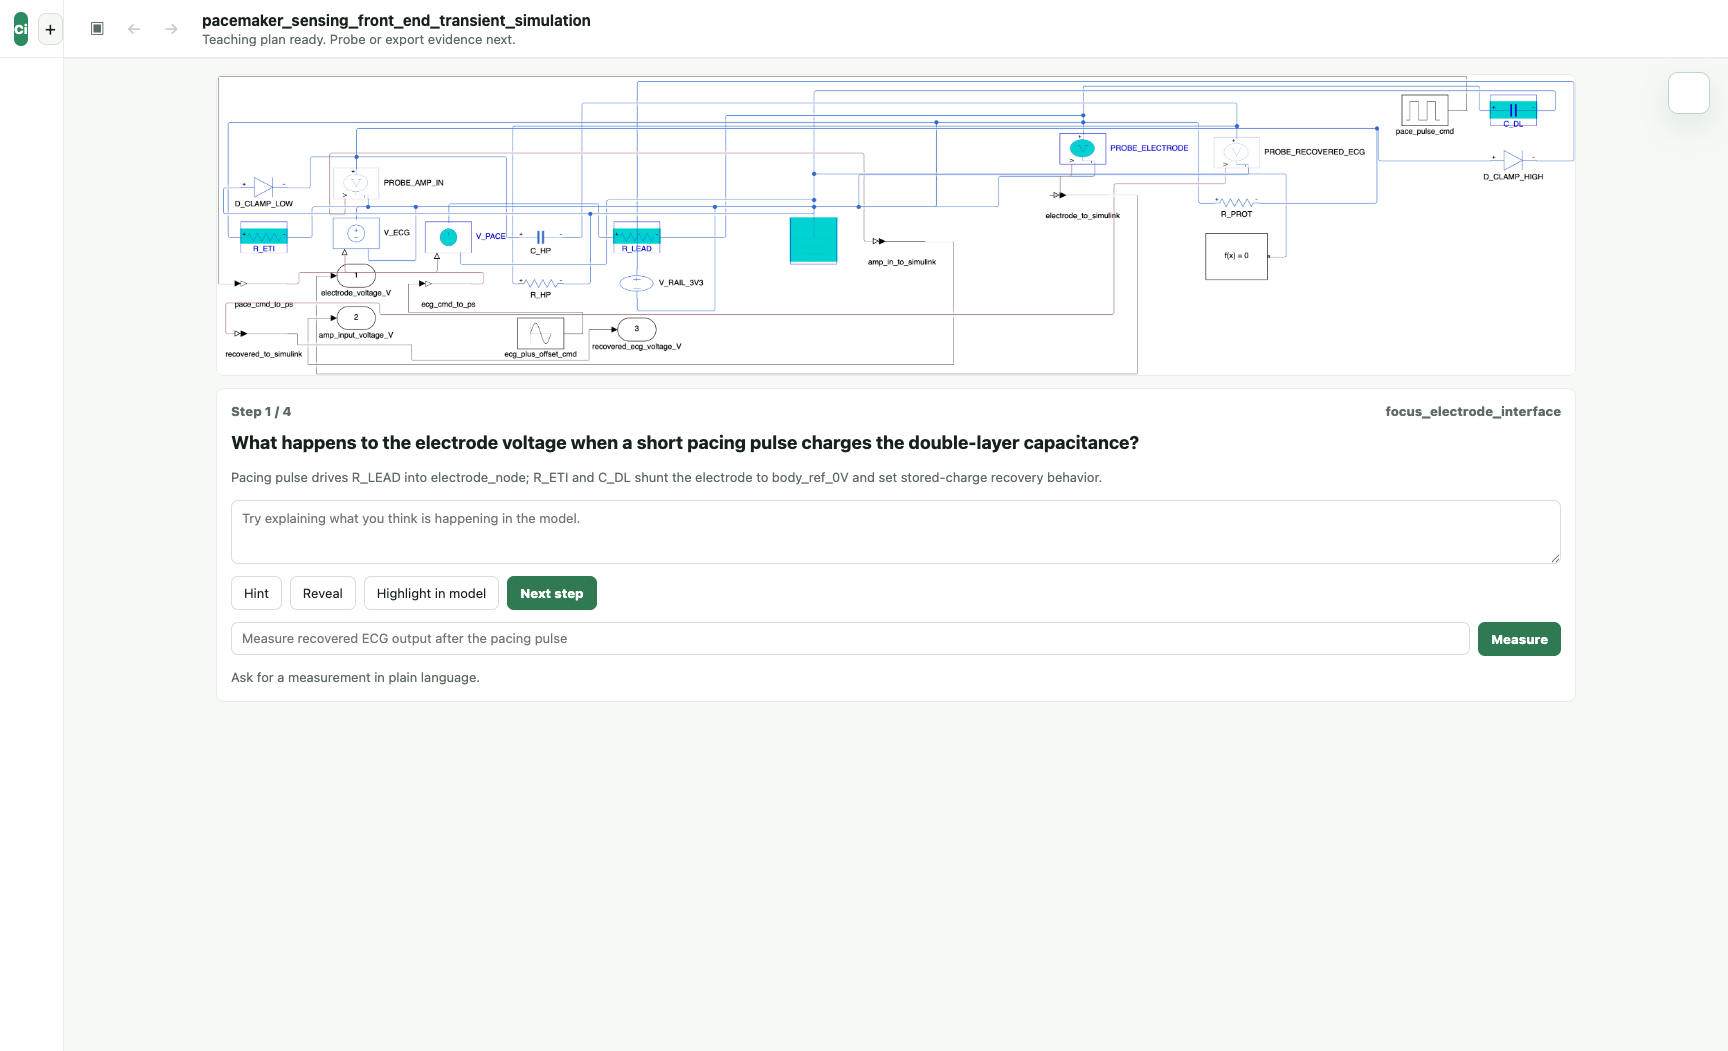
\includegraphics[width=0.31\textwidth]{figures/fig2_app_open.png} &
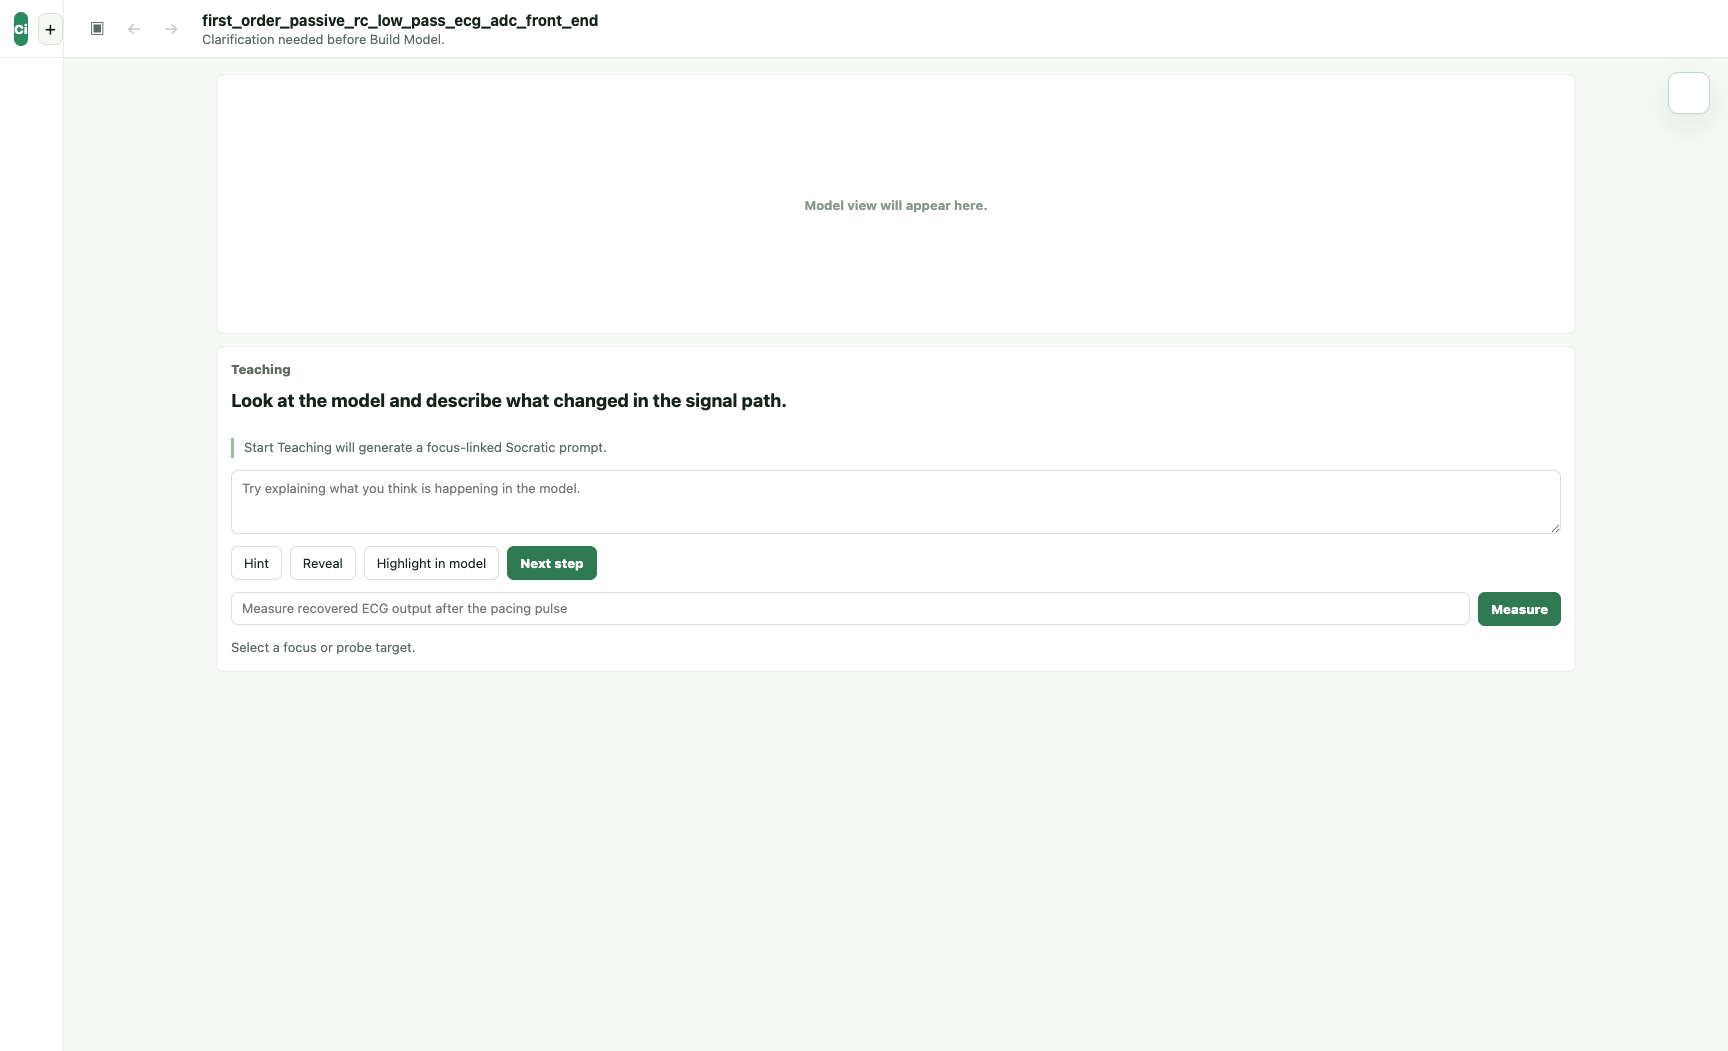
\includegraphics[width=0.31\textwidth]{figures/fig2_read_page.png} &
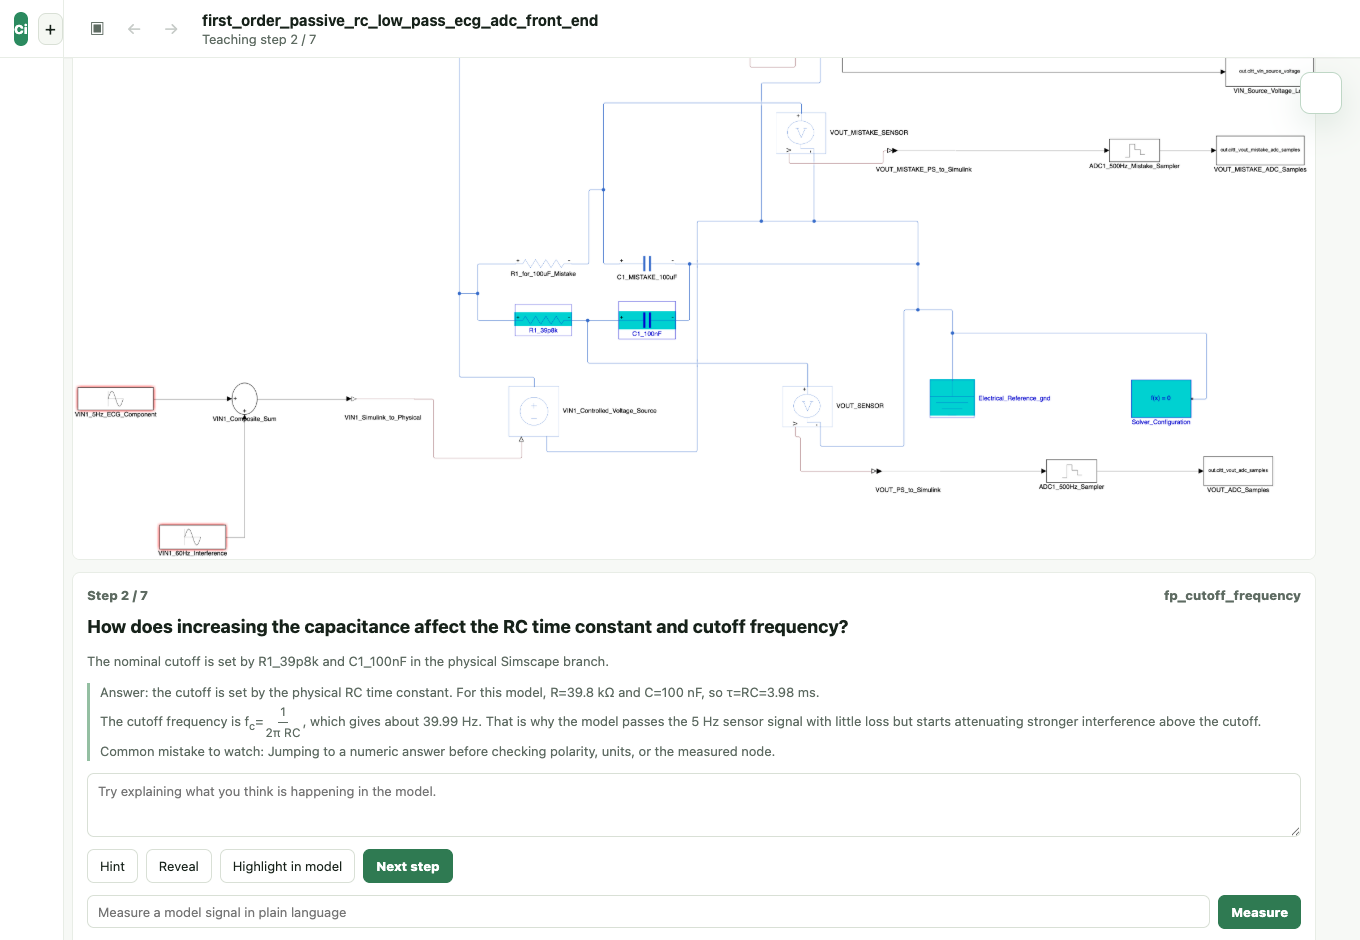
\includegraphics[width=0.31\textwidth]{figures/fig2_teach_page.png} \\
(a) App launch & (b) Read/parse stage & (c) Teaching/probe surface
\end{tabular}
\caption{MATLAB/CiTT UI evidence from the live GUI pass. The release UI is a MATLAB-native, model-centered learning surface rather than the older web-first prototype.}
\label{fig:ui}
\end{figure*}

The system has five main components. The parser converts circuit images or text prompts into structured specifications. The model-building layer prepares tasks for SATK/MCP-compatible agents and validates produced models, focus maps, probe maps, and reports. The UI opens or previews Simulink/Simscape artifacts and keeps the model visually central. The teaching layer builds Socratic steps from focus maps and links explanation to highlights. The probe/evidence layer records measurement targets, model checks, simulation summaries, plots, and exported evidence packs.

The release package includes only the MATLAB plugin, resources, schemas, prompts, and setup/demo documentation. It excludes \texttt{.env} files, API keys, \texttt{matlab/work/}, Simulink caches, and old offline evidence. A post-package verification script installed the toolbox, launched the GUI, and reproduced the three examples under \texttt{release/example\_repro/}.
